\section{Evaluation}
\subsection{Prüfung der Anforderungen}%Anforderungserfüllung}

Dieser Abschnitt behandelt in wie weit das beschriebene Konzept die in Kapitel 1 aufgelisteten Anforderungen erfüllt. Die jeweilige Anforderung wird zunächst wiederholt und anschließend genauer untersucht.

\subsubsection{Transparente Einzahlungen}
Die Einzahlung jedes Endnutzers ist für jeden anderen Endnutzer nachprüfbar.\\\\
Diese Anforderung ist erfüllt, da jede Transaktion in der lokalen Datenbank jedes Peet-to-Peer Netzwerkteilnehmers aufgezeichnet wird. 
Auf der Webseite \cite{blockchain_info} kann man die Bitcoin Blockchain mithilfe eines sogenannten Blockchain-Exploers durchsuchen. Mit diesem Werkzeug kann man die Blöcke und die darin enthaltenen Transaktionen untersuchen. Nutzt man den Explorer einer Drittpartei, muss man darauf vertrauen, dass dieser auch den ''wahren'' Status der Blockchain anzeigt. Um dieses Risiko zu vermeiden kann jeder Teilnehmer mithilfe eines eigenen Bitcoin Full Node am Netzwerk teilnehmen. Dieser speichert die gesamte Blockchain und prüft alle Transaktionen und Blöcke gegen die Konsensregeln.\\
Der Bitcoin Full Node stellt eine API bereit, über die man den aktuellen Status der Blockchain abfragen kann. Der Befehl \textbf{getblockchaininfo} liefert den aktuellen Zustand der Blockchain zurück. Dieser beinhaltet die Blocknummer des neusten Blocks und dessen Blockhash. Der Befehl \textbf{gettransaction} gefolgt von der Transaktions-ID liefert Details über eine Transaktion. Die Webseite \cite{btc_api} dokumentiert diese Schnittstelle detailliert. 

\subsubsection{Gewinnerauswahl durch Zufallsfaktor}
Die Auswahl des Gewinners ist von einem zufälligen Faktor abhängig, auf den weder die Anwendung noch die Endnutzer einen Einfluss haben.\\\\
Diese Anforderung wird nur bedingt erfüllt, da ein Teilnehmer des Peer-to-Peer Netzwerks sowohl ein Spieler als auch ein Miner sein kann. Ist dies der Fall besteht die Möglichkeit, dass der Miner einen validen Blockhash verwirft, sobald er merkt, dass er durch diesen Blockhash nicht zum Gewinner des Geldtopfes wird. Verwirft der Teilnehmer einen Blockhash, riskiert er den dadurch ausgeschütteten Blockreward. Ein solcher Angriff ist für einen Miner nur rentabel, falls die Spieleinsätze des Geldtopfes den Blockreward um ein vielfaches übersteigen.
Betrachten wir dazu das Bitcoin Netzwerk Anfang Februar 2018. Der Preis pro Bitcoin beträgt 8000 Euro. Der Mining Reward liegt bei 12,5 Bitcoin pro Block. Für das Lösen eines gültigen Blocks erhält ein Miner somit 100000 Euro. Angenommen ein Miner besitzt 20 Prozent der Hashrate des gesamten Bitcoin-Netzwerks und nimmt an einem Topf mit 2 Personen teil. Dies bedeutet, dass sowohl der Miner als auch der andere Teilnehmer eine Gewinnwahrscheinlichkeit von 0,5 für einen zufälligen Blockhash haben.
Da der Miner eine Hashrate von 20 Prozent hat, liegt die Wahrscheinlichkeit das der Miner den nächsten Block findet bei 0,2. Falls er den gefundene Blockhash verwirft, da er durch diesen seinen Glücksspieleinsatz verlieren würde, muss er es schaffen vor einem anderen Miner einen weiteren Blockhash zu berechnen. Ansonsten verliert er den Blockreward. Die Wahrscheinlichkeit das der Miner zwei gültige Blockhashs hintereinander findet, liegt bei 0,2 * 0,2 = 0,04 und ist somit verschwindend gering.

\subsubsection{Nachprüfbarkeit des Zufallsfaktor}
Jeder Endnutzer kann die Echtheit des zufälligen Faktors eigenständig nachprüfen.\\\\
Da das Verfahren der Gewinnerauswahl im Vorhinein festgelegt ist und die Reihenfolge der Einzahlungstransaktionen in der Blockchain festgeschrieben steht, kann jeder Teilnehmer die Berechnung des Gewinners eigenständig nachvollziehen. Der Blockhash der die Grundlage für die Gewinnerauswahl liefert kann durch die Verwendung eines Bockchain-Explorers oder eines Full Nodes nachgeprüft werden. 
\subsubsection{Transparente Auszahlungen}
Die Auszahlung an den Gewinner muss transparent und somit für jeden Endnutzer nachprüfbar sein.\\\\
Genau wie die Einzahlungen ist auch die Auszahlung für jeden Spieler mithilfe eines Blockchain-Explorers oder eines Bitcoin Full Nodes möglich. Jeder Teilnehmer kann somit für alle bereits abgeschlossenen Spiele nachprüfen ob die Anwendung sich korrekt verhalten und eine Auszahlung getätigt hat. 
\subsubsection{Fairheit des Spiels}
Jeder Endnutzer besitzt die gleiche Gewinnwahrscheinlichkeit und niemand wird benachteiligt.\\\\
Die Zuordnung der Spieler auf die Gewinnzahlen ist durch die Reihenfolge der Transaktionen in der Blockchain festgeschrieben. Eine nachträgliche Veränderung dieser Reihenfolge ist weder durch die Nutzer, noch durch die Glücksspielanwendung möglich.\footnote{Eine Veränderung der Reihenfolge ist nur durch einen sogenannten Blockchain-Fork möglich. Kapitel \ref{Chapter6} erörtert welche Auswirkungen dies auf die Glücksspielanwendung hat.}

Damit keiner der Spieler einen Vorteil hat, muss jeder Topf-Platz die gleiche Gewinnwahrscheinlichkeit haben.
Dies ist gegeben, falls a) jeder Teilnehmer die gleiche Anzahl Gewinnzahlen zugeordnet bekommt und b) falls die möglichen Blockhash-Werte für die Gewinnerauswahl gleichverteilt sind.\\

a) Die Gewinnerauswahl kann entweder wie im Konzept beschrieben durch den gesamten Blockhash-Wert oder wie im Beispiel auf Basis der letzten Blockziffer vorgenommen werden.
Beide Methoden haben Vor- und Nachteile.\\ Variante eins erlaubt beliebige Topfgrößen, ist dafür aber schwieriger für den Endnutzer zu verifizieren. Die Verifizierung erfordert die Konvertierung des Blockhashs ins Dezimalsystem und eine Modulo-Rechnung einer sehr große Zahl.\\ Variante zwei ist dagegen leicht zu verifizieren, erlaubt allerdings nur die Topfgrößen zwei, fünf und zehn. Bei der Topfgröße von zwei sind beiden Spielern fünf Gewinnzahlen zugeordnet. Bei der Topfgröße von fünf besitzt jeder Teilnehmer genau 2 Gewinnzahlen. Bei einer Topfgröße von zehn wird jedem Teilnehmer genau eine Gewinnzahl zugeordnet. 
Nimmt man hingegen eine Topfgröße von 1,3,4,6,7,8 und 9 führt dies dazu das manche Teilnehmer eine signifikant höhere Gewinnchance haben.
Bei der Topfgröße von 3 sind die Gewinnzahlen durch die Modulo-Funktion folgendermaßen verteilt:
\begin{itemize}
\item Spieler 1 hat die Gewinnzahlen 0, 3 und 9.
\item Spieler 2 hat die Gewinnzahlen 1 und 4.
\item Spieler 3 hat die Gewinnzahlen 2, 5 und 8.
\end{itemize}
Somit haben Spieler 1 und 3 eine Gewinnwahrscheinlichkeit von $\frac{3}{10}$, Spieler 2 hingegen nur eine Gewinnwahrscheinlichkeit von $\frac{2}{10}$.

Es kommt also vor, dass eine Teilmenge der Spieler genau eine Gewinnzahl mehr als der Rest der Teilnehmer hat.
Nimmt man den gesamten Blockhash zur Gewinnerauswahl ist die dadurch entstehende Ungerechtigkeit verschwindend gering und kann vernachlässigt werden. Dies ist der Fall, da die aus dem Blockhash resultierende Dezimalzahl in der Praxis sehr groß ist und jeder Spieler somit mehrere Millionen von Gewinnzahlen hat.\\

b) Der Blockhash eines Blocks wird durch die verwendete kryptographische Hashfunktion der Kryptowährung festgelegt. Die Verteilung der Werte ist somit von der verwendeten kryptographische Hashfunktion abhängig.\\
Eine kryptografische Hashfunktion ist eine stark kollisionsresistente Einweg-Hashfunktion.\\
Eine Hashfunktion h heißt
\begin{itemize}
\item Einwegfunktion genau dann, wenn es schwierig ist, zu gegebenem $_{Y0}$ ein $_{X0}$ zu finden mit $h(x_{0}) = y_{0}$.
\item schwach kollisionsresistent genau dann, wenn es schwierig ist, zu einem gegebenen $x$ ein $x'$ zu finden mit $h(x) = h(x')$.
\item stark kollisionsresistent genau dann, wenn es schwierig ist, $x$ und $x'$ zu finden
mit $x \neq xx$ und $h(x) = h(xx)$.
\end{itemize}Die Eigenschaften der starken Kollisionsresistenz und der Einwegfunktion sagen nichts über die Verteilung der ausgegebenen Werte aus. Bei der Auswahl der Kryptowährung muss also gesondert auf die Verteilung der verwendete Hashfunktion geachtet werden. Sollte die verwendete kryptographische Hashfunktion keine Gleichverteilung liefern, kann der Blockhash dennoch den nötigen Zufall liefern indem dieser mit einer geeigneten Hashfunktion erneut gehasht wird.\\\\
Bitcoin verwendet die kryptographische Hashfunktion SHA256.
Die folgende Monte-Carlo-Simulation zeigt, dass die Resultate der SHA256 gleichverteilt sind.
\begin{verbatim}
h=SHA256 n=1000000
for i 1 -> n
    hash = h(i);
    result[lastDigit(hash)]++
\end{verbatim}
\begin{minipage}{0.5\textwidth}
\begin{verbatim}
Ausgabe:
result[0] =  99765
result[1] = 100488
result[2] =  99913
result[3] = 100745
result[4] = 100272
result[5] =  99649
result[6] =  99430
result[7] =  99788
result[8] =  99666
result[9] = 100284
\end{verbatim}
\end{minipage}
\begin{minipage}{0.5\textwidth}
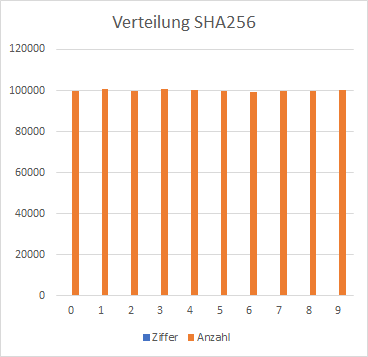
\includegraphics[width=\textwidth]{Figures/verteilung_sha256}
\centering
\decoRule
\captionof{figure}{\label{fig:verteilung_sha256}Verteilung der SHA256 Hashfunktion}
\label{fig:verteilung_sha256}
\end{minipage}

\pdfcomment{Hier dann noch die Verteilung der echten Bitcoin Blockchain angeben.}
%Somit ist das Spiel nur unter der Annahme fair, dass die Zahl zur Gewinnerauswahl gleichverteilt ist.

\subsection{Betrugsmöglichkeiten}

Dieser Abschnitt betrachtet in wie weit die Glücksspielanwendung potentielle Spieler betrügen kann, sollte sie gehackt und zu ausschließlich diesem Zweck modifiziert werden.
Die Anwendung hat die volle Kontrolle darüber welche Ausgabe sie dem Benutzer anzeigt. Sie hat allerdings keine Kontrolle über den Status der Blockchain. 

Die Anwendung könnte beispielsweise anzeigen, dass der Topf nach der Einzahlung durch einen Spieler immer noch leer ist. Die Transaktion auf die Einzahlungsadresse existiert dann zwar in der Blockchain allerdings reagiert die Anwendung nicht entsprechend. Dies hat zur Folge, dass jeder Spieler der eine Einzahlung tätigt, sein Geld verliert. Allerdings merkt der Benutzer dies und kann somit eine weitere Verwendung der Anwendung unterlassen. Ein solch plumper Manipulationsversuch fällt somit direkt auf.

Ein weitere Betrugsmöglichkeit ist, dass die Glücksspielanwendung sich bis zur Gewinnerauswahl korrekt verhält, dann allerdings keine Auszahlung tätigt. Alle einzahlenden Spieler merken den Betrug, verlieren aber dennoch ihr Geld.

Bei beiden vorgestellten Betrugsversuchen fällt der Betrug immer mindestens einem Spieler auf. Die Verwendung einer solchen Anwendung macht nur Sinn, falls man den Betreiber des Services kennt und diesen im Zweifel juristisch haftbar machen kann.\\
Das folgende Kapitel betrachtet wie sogenannte ''Smart Contract''s dieses Problem lösen. Ein Smart Contract erlauben es die Geschäftslogik der Glücksspielanwendung in die Blockchain zu schreiben. Die Geschäftslogik wird somit nicht mehr von der Anwendung, sondern von jedem Teilnehmer des Peer-to-Peer Netzwerks ausgeführt. 


\subsection{Angriff durch Miner}

\pdfcomment{Überlegungen wie man es nicht machen kann:Blockhash 100 mal hashen bringt nicht. Miner findet Hash und macht erst danach die Arbeit. Die 5 letzten Blockhashs mit einbeziehen bringt auch nichts, weil es dann nur auf den 5. letzten Block ankommt}

\subsection{Blockchain Mining Varianz}

\pdfcomment{Hier gibt es einen Vorschlag, wie man die erhoffte Blocktime öffters erreichen kann.
Bobtail: A Proof-of-Work Target that Reduces Blockchain Mining Variance (Brian N. Levine)
https://stanford2017.scalingbitcoin.org/presentations}

\subsection{Auszahlungstransaktion}
Die Glücksspielanwendung erzeugt für jede Einzahlung eine eigene Einzahlungsadresse statt für jeden Benutzer die gleiche Adresse zu verwenden. Dies hat den Vorteil, dass die Anwendung dem Benutzer anzeigen kann, dass sein Bitcoin Einzahlung eingegangen ist. Der Nachteil ist, dass dadurch die Größe der Auszahlungstransaktion steigt und man somit eine höhere Transaktionsgebühr zahlen muss. Im folgenden wird die Auszahlungstransaktion des Beispiels aus \ref{ssec:btc_gui} betrachtet.

\begin{figure}[H]
\centering
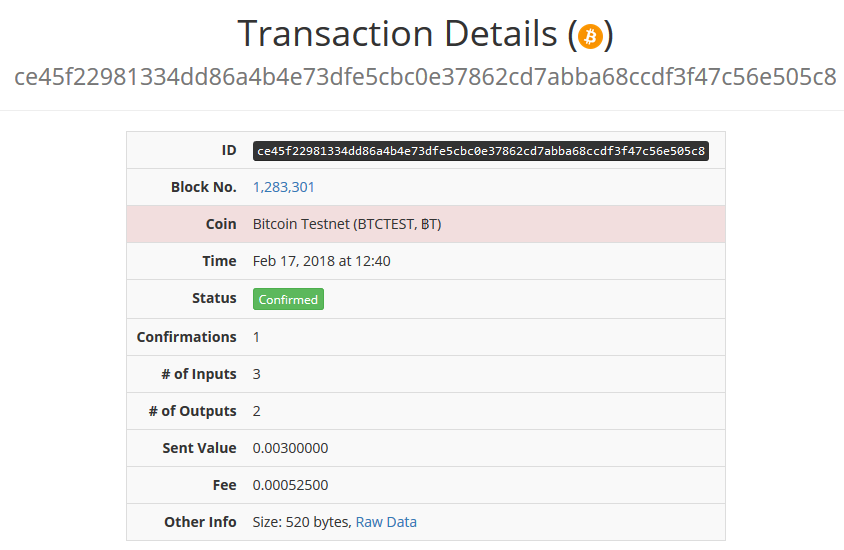
\includegraphics[width=1\linewidth]{Figures/btc_gui/btc_txn}
\decoRule
\caption{Auszahlungstransaktion Details}
\label{fig:btc_txn}
\end{figure}

\label{fig:btc_txn} zeigt in welchen Block die Transaktion aufgenommen wurde. Den Status, den Wert, die Transaktionsgebühr und die Größe der Transaktion.
\footnote{Momentan zahlt die Glücksspielanwendung die Auszahlungstransaktionsgebühr aus eigener Tasche. Eigentlich müsste die Transaktionsgebühr von dem Gewinnbetrag abgezogen werden.}

\begin{figure}[H]
\centering
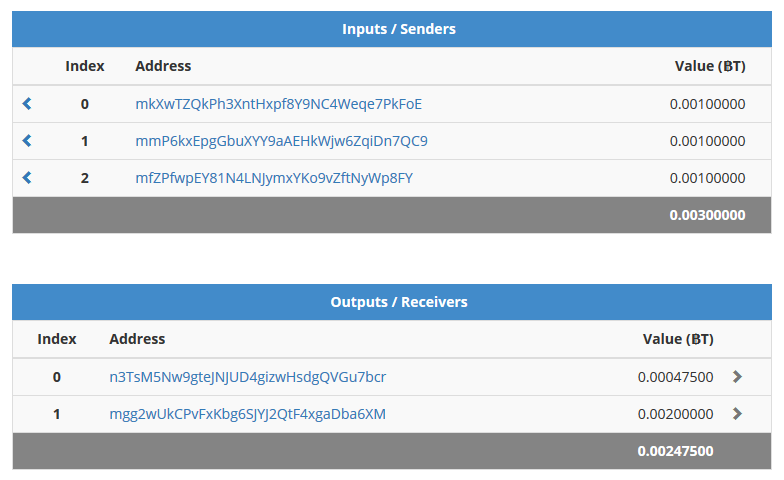
\includegraphics[width=1\linewidth]{Figures/btc_gui/btc_txn_input_output}
\decoRule
\caption{Auszahlungstransaktion Inputs und Outputs}
\label{fig:btc_txn_input_output}
\end{figure}


\label{fig:btc_txn_input_output} zeigt welche Inputs und Outputs für die Transaktion verwendet wurden. Output Adresse 0 gehört dem Wallet der Glücksspielanwendung und stellt die Wechselgeldadresse dar.


\begin{figure}[H]
\centering
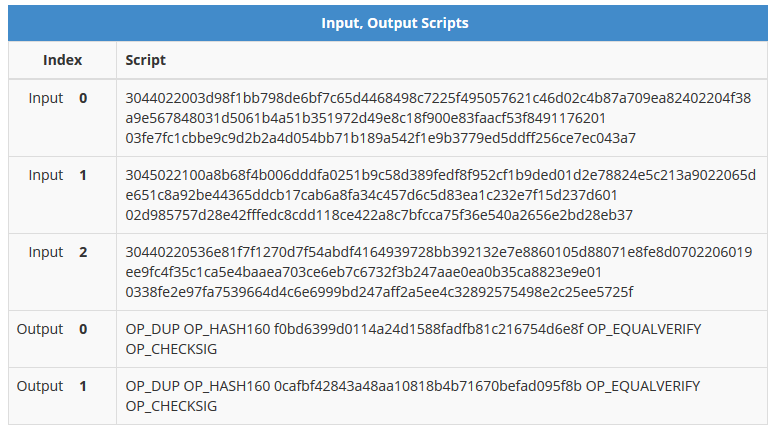
\includegraphics[width=1\linewidth]{Figures/btc_gui/btc_txn_input_output_scripts}
\decoRule
\caption{Auszahlungstransaktion Skripts}
\label{fig:btc_txn_input_output_scripts}
\end{figure}

Da die Anwendung für jeden Benutzer eine eigene Adresse generiert, muss die Anwendung in der Auszahlungstransaktion für jede Input Adresse eine gültige Signatur angeben.\label{fig:btc_txn_input_output_scripts} zeigt, dass die Transaktion dadurch wesentlich größer wird. Hier könnte in Zukunft die Verwendung sogenannter Schnorr Multi-Signaturen aushelfen. Durch diese lassen sich alle Signaturen der Inputs durch eine einzige Signatur ersetzen.